\documentclass[landscape, 12pt]{report}

\usepackage{ptext}
\usepackage{lipsum}
\input{Boostan-UserManual}
\usepackage{graphicx}
\usepackage{tabularx}


\newword{Abstraction}{Abstraction}
{انتزاع}{}

\newword{Abstract}{Abstract}
{انتزاعی}{}

\newword{AbsoluteMinimum}{Absolute Minimum}
{کمینه مطلق}{}


\newword{AcceptableCell}{Acceptable Cell}
{سلول پذیرفتنی}{سلول‌های پذیرفتنی}

\newword{AccessBurst}{Access Burst}
{توده دسترسی}{توده‌های دسترسی}


%%% S
\newword{Sample}{Sample}
{نمونه}{نمونه‌ها}

\newword{SamplePath}{Sample Path}
{نمونه مسیر}{}

\newword{SampleSpace}{Sample Space}
{فضای نمونه}{فضای نمونه‌ها}
\newacronym{ACK}{ACK}{Acknowledgement}

\newacronym{ACI}{ACI}{Application Control Interface}

\newacronym{ACIR}{ACIR}{Adjacent Channel Interference Ratio}

\newacronym{ACLC}{ACLC}{Adaptive Configuration of Logical Channels}

\newacronym{ACLP}{ACLP}{Adjacent Channel Leakage Power}

\title{مفهوم
	ORAN
	در شبکه های نسل پنج
}
\type{
 درس آشنایی با شبکه های تلفن همراه }
\author{غزل عربعلی - 97521396، بهاره کاوسی نژاد - 99431217}
\logofile{Pic/IUST}


\begin{document}



\pagenumbering{gobble}
\maketitle
\pagenumbering{arabic}
\chapter*{مقدمه}

\section*{تحولی در معماری
	  \lr{RAN}
	  }
به شکل \ref{fig:site} سایت می گویند. سایت ها برای ارائه پوشش بی سیم
 (
 \lr{Wireless Coverage}
 ) به کاربران در یک منطقه جغرافیایی خاص قرار می‌گیرند.
\begin{figure}[ht]
	\centering
	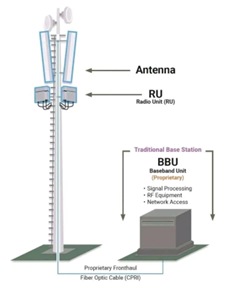
\includegraphics[height=.3\linewidth]{Pic/Picture1}
	\caption{سایت}
	\label{fig:site}
\end{figure}
قرار گیری مولفه های
 \lr{RAN}
   مانند سایت که شامل سلول های زیادی است برای اطمینان از دسترسی قابل اعتماد و ثابت             (
   \lr{Reliable \& Consistent}
   ) کاربران به خدمات شبکه بسیار مهم است. به همین جهت هنگام برنامه ریزی برای استقرار شبکه دسترسی رادیویی، اپراتورهای شبکه عوامل مختلفی را در نظر می گیرند مانند
   \begin{itemize}
   	\item تراکم جمعیت،
   	\item توپوگرافی که به معنای ویژگی ها و خصوصیات سطح زمین در یک منطقه خاص است،
   	\item تراکم ساختمان ها و
   	\item الگوهای ترافیکی در یک منطقه تحت پوشش
   \end{itemize}
چرا که به طور مثال برای دسترسی بهتر کاربران با توجه به آرایش ترافیکی گاهاً به صورت داینامیک
 \lr{Config}
  شبکه را در طول روز تغییر می‌دهند. با تحلیل پارامترهای نام برده شده و دیگر پارامترها اپراتور های شبکه می توانند مکان بهینه و پیکربندی
   \lr{RAN}
    را  با هدف پوشش و ظرفیت حداکثری تعیین کنند. به طور کلی مکان قرارگیری
     \lr{RAN}
      کارایی کلی شبکه را نیز تحت تاثیر قرار می‌دهد.در نتیجه برای داشتن پوشش دهی و
       \lr{Mobility}
        باید از استراتژی برای قرار دادن
         \lr{RAN}
          استفاده کنیم.


\chapter*{اجزای شبکه مخابرات بی سیم}
اجزای شبکه مخابرات بی سیم از ۳ جزء اصلی تشکیل شده است (شکل \ref{fig:Wireless_Telecommunications_Systems}) که یکی
 \lr{User Terminal}
   یا
  \lr{User Equipment}
   و یا
    \lr{Mobile Station}
     که در نسل ۲ از این اصطلاح استفاده می شد، دیگری
      \lr{RAN}
        و آخرین جزء
         \lr{Core Network}
          خواهد بود.
          
          
\begin{figure}[ht]
	\centering
	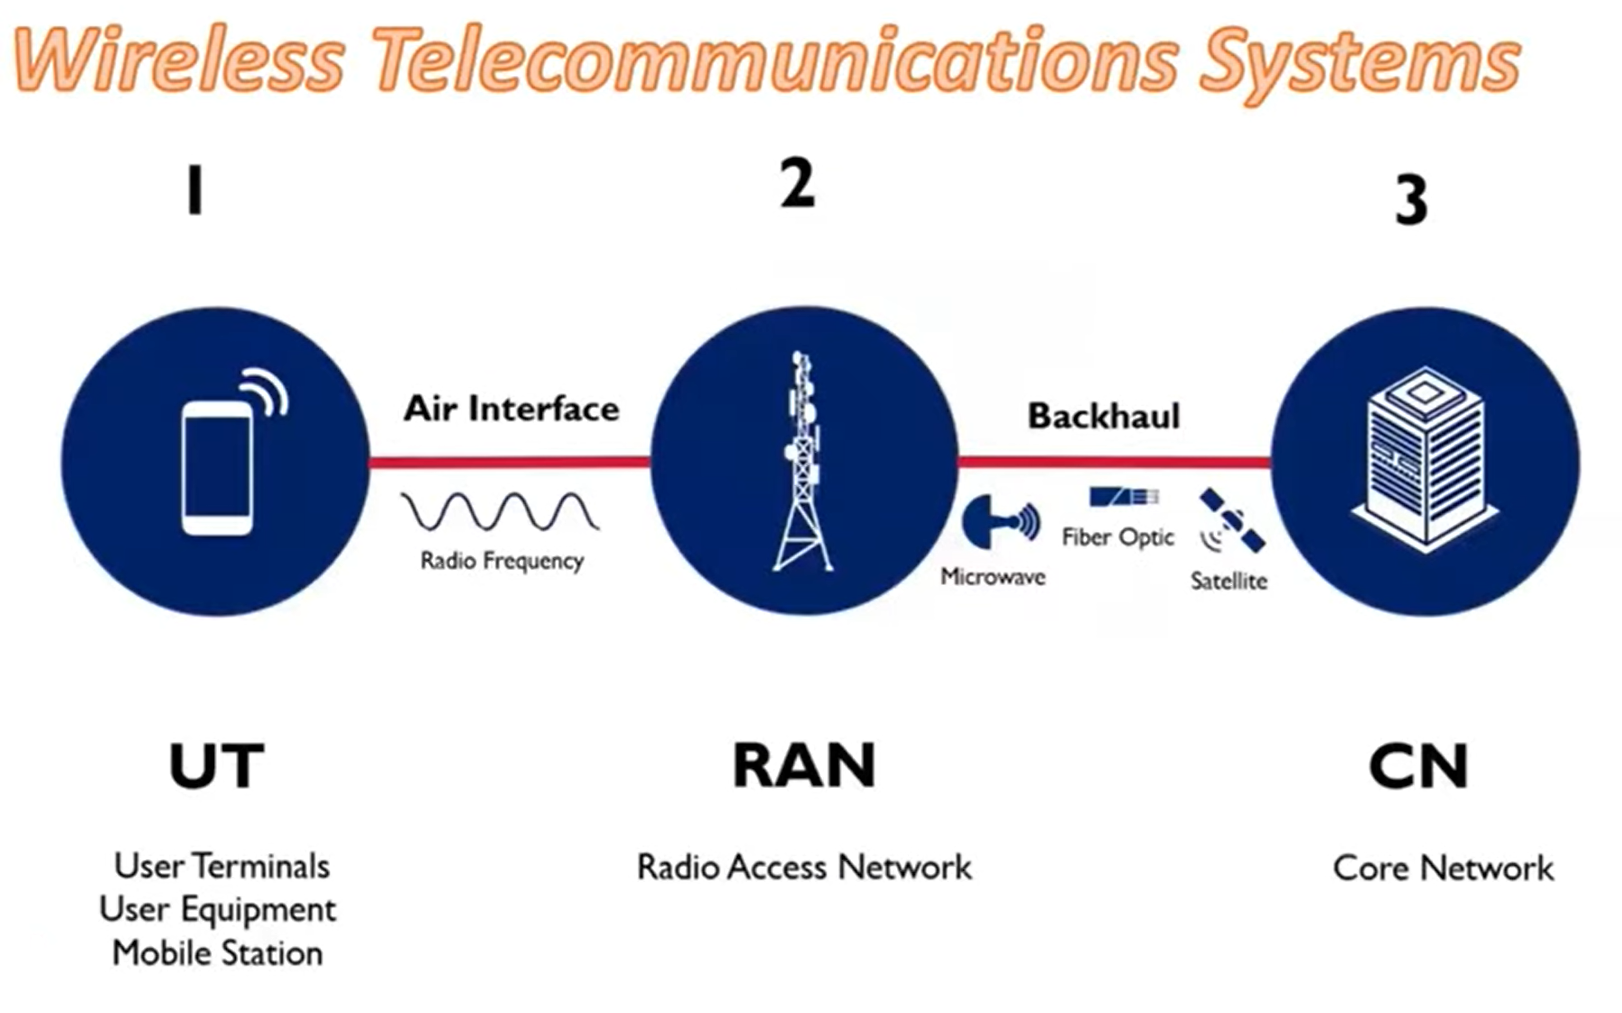
\includegraphics[width=.6\linewidth]{Pic/Wireless_Telecommunications_Systems}
	\caption{اجزای شبکه مخابرات بی سیم}
	\label{fig:Wireless_Telecommunications_Systems}
\end{figure}
وظیفه ناحیه
 \lr{RAN}
  فراهم کردن ارتباط یا
   \lr{Connection Stable}
    برای دستگاه های تلفن همراه است. اگر بخواهیم از ۳ جزء اصلی در
     \lr{Traditional RAN}
      ها نام ببریم میتوان از آنتن،
       \lr{RRU}
        و
         \lr{BBU}
          نام برد. ارتباط میان
            \lr{user terminal}
             و ناحیه
              \lr{RAN}
               از طریق
               \lr{air interface}
                و به صورت
                  \lr{wireless}
                   و با استفاده از پروتکل
                    \lr{AS(Access Stratum)}
                     است که در دیالوگ ها و ارتباط میان دیوایس‌ها و زیر ساخت رادیویی شبکه من جمله
                      \lr{eNodeB}
                       در نسل ۴ و
                        \lr{gNodeB}
                         در نسل ۵ به کار می‌رود . از مجموعه فرکانس های مختلفی جهت برقراری این ارتباط میان ناحیه
                          \lr{RAN}
                           و
                            \lr{User Terminal}
                             استفاده می‌شود که آن را فرکانس رادیویی می‌خوانیم. ناحیه
                              \lr{RAN}
                               از طریق لینک
                                \lr{backhaul}
                                که ترافیک داده از
                                 \lr{RAN}
                                  را به هسته شبکه منتقل می‌کنند به 
                                  \lr{Core Network}
                                   متصل شده اند. 
هسته شبکه وظایف مختلف و مهمی را بر عهده دارد من جمله
 \lr{Routing}
  بین شبکه‌های مختلف،
   \lr{Call}
   ،
    \lr{Message}
    ،
     \lr{USSD}
     ،
      \lr{Internet}
       و به صورت کلی
        \lr{data service}
         ها و ۳ راه اتصال
          \lr{RAN}
           به
            \lr{Core Network}
             وجود دارد که می‌تواند
              \lr{fiber optic}
               یا
                \lr{microwave}
                 باشد و اگر مشکلاتی از در فاصله زیاد و انحنای زمین و ... وجود دارد میتوان از 
                 \lr{Satellite}
                   استفاده کرد.


\section*{بررسی 
\lr{RAN}
به صورت دقیق تر
}
حال به بحث دقیق تر درباره
 \lr{RAN}
  می
  پردازیم:
مکان قرارگیری این ناحیه به صورت خیلی گسترده ای توزیع شده است. چرا در که تمامی نواحی وظیفه برقراری ارتباط و پوشش دهی بدون وقفه و اختلال را دارد.
این ناحیه به طور مداوم از نسل اول تا نسل پنجم تکامل یافته است اما برخی از اجزای ضروری آن باقی مانده اند مانند آنتن که سیگنال الکتریکی را به امواج رادیویی تبدیل می‌کند و بالعکس.
 \lr{RU}
  یا
   \lr{Radio Unit}
    که وظیفه آن استفاده از باند های فرکانسی و سطوح توان مناسب است.
     \lr{BBU}
      یا
       \lr{BaseBand Unit} 
       که سیگنال هارا پردازش می‌کند و این بخش شامل واحد های نرم‌افزاری و سخت‌افزاری جهت برقراری ارتباط بی‌سیم از طریق امواج رادیویی است.
برای ناحیه
 \lr{RAN}
  در نسل های مختلف نامگذاری ها متفاوتی وجود دارد که در تصویر \ref{fig:RAN_Generations} مشاهده می‌کنیم. همان طور که دیده می شود، در نسل پنج، به آن 
  \lr{NG-RAN}
  (
  \lr{New}
  	یا
  	\lr{Next Generation RAN}
  )
  می گویند.
  \begin{figure}[ht]
  	\centering
  	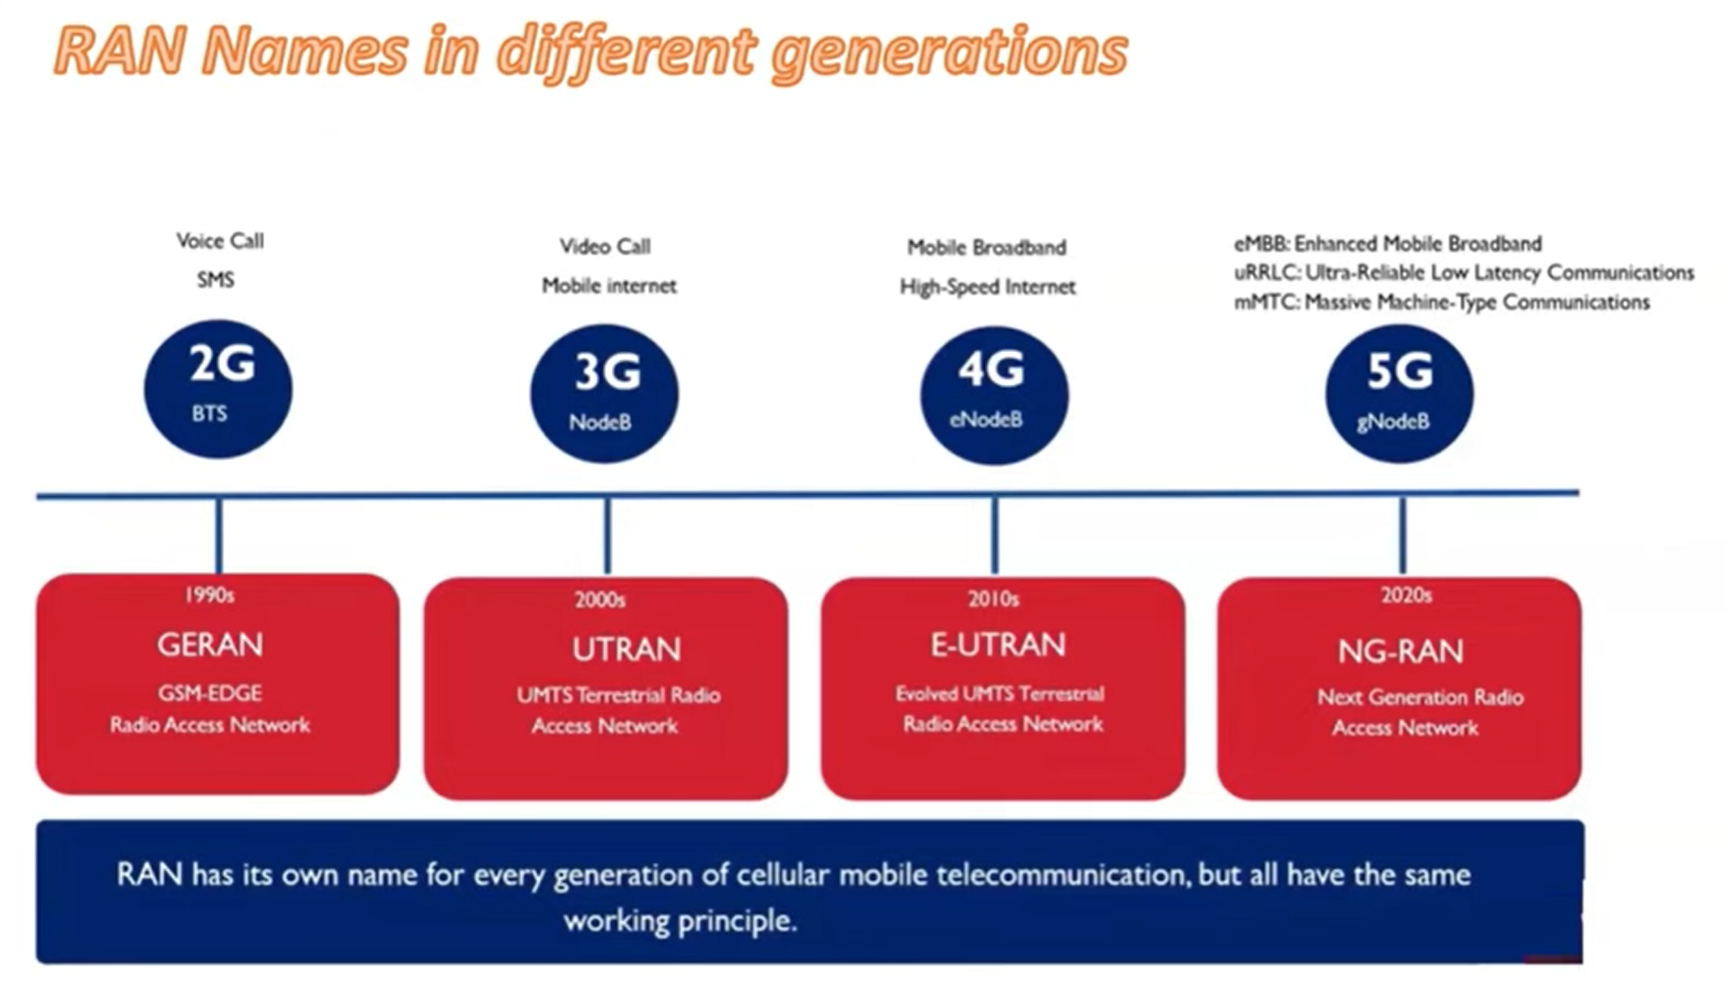
\includegraphics[width=.6\linewidth]{Pic/RAN_Generations}
  	\caption{نسل های مختلف
  		\lr{RAN}
  	}
  	\label{fig:RAN_Generations}
  \end{figure}
  
  همانطور که در شکل \ref{fig:Baseband_Unit} دیده می شود، در 
  \lr{Traditional RAN}
  ،
   \lr{Baseband}
     در زیر برج مانندی قرار دارد و روی برج
      \lr{RRU}
       و آنتن نصب شده‌اند. و این واحد مسئولیت سیگنال های
        \lr{Baseband}
         را بر عهده دارد و در یک کابینی به نام
          \lr{Equipment Room}
           قرار دارد و به وسیله فیبر نوری به
            \lr{RRU}
             که روی برج مانند نصب شده است متصل می‌شود. 
 \begin{figure}[ht]
 	\centering
 	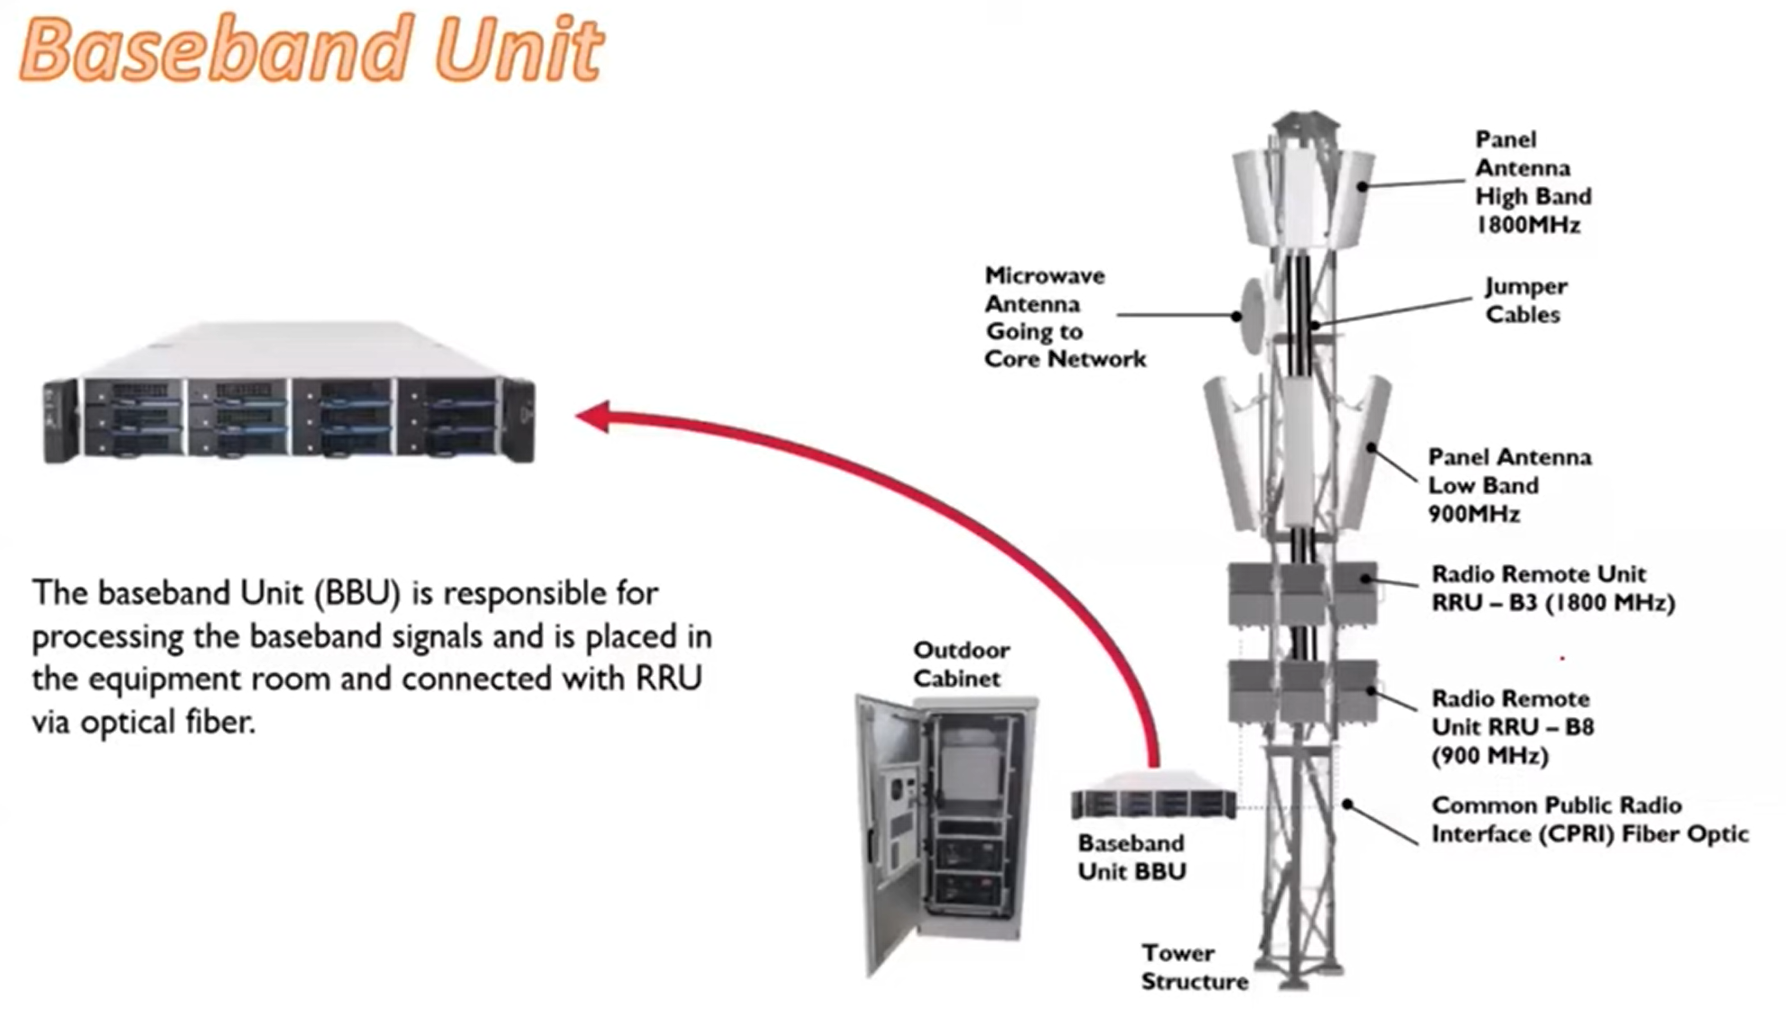
\includegraphics[width=.6\linewidth]{Pic/Baseband_Unit}
 	\caption{
 	\lr{Baseband}
 	در
 	\lr{Traditional RAN}
 	}
 	\label{fig:Baseband_Unit}
 \end{figure}

\section*{واحد
\lr{RRU}
}
واحد
 \lr{RU}
  یا
   \lr{RRU}
   (شکل \ref{fig:RRU}) روی برج نصب شده است . رابطی سریال به نام
     \lr{CPRI}
      ( 
    \lr{Common Public Radio Interface}
    ) که در شکل \ref{fig:CPRI} مشاهده می شود، انتقال داده ها با سرعت بالا از طریق کابل فیبر نوری را فراهم می‌سازد. درنتیجه از طریق آن تمامی سیگنال های رادیویی به
     \lr{function}
      محاسباتی (
       \lr{Computing Function}
       ) که در
        \lr{Base Band Unit}
         وجود دارد منتقل می‌شوند.
   
\begin{figure}[ht]
	\centering
	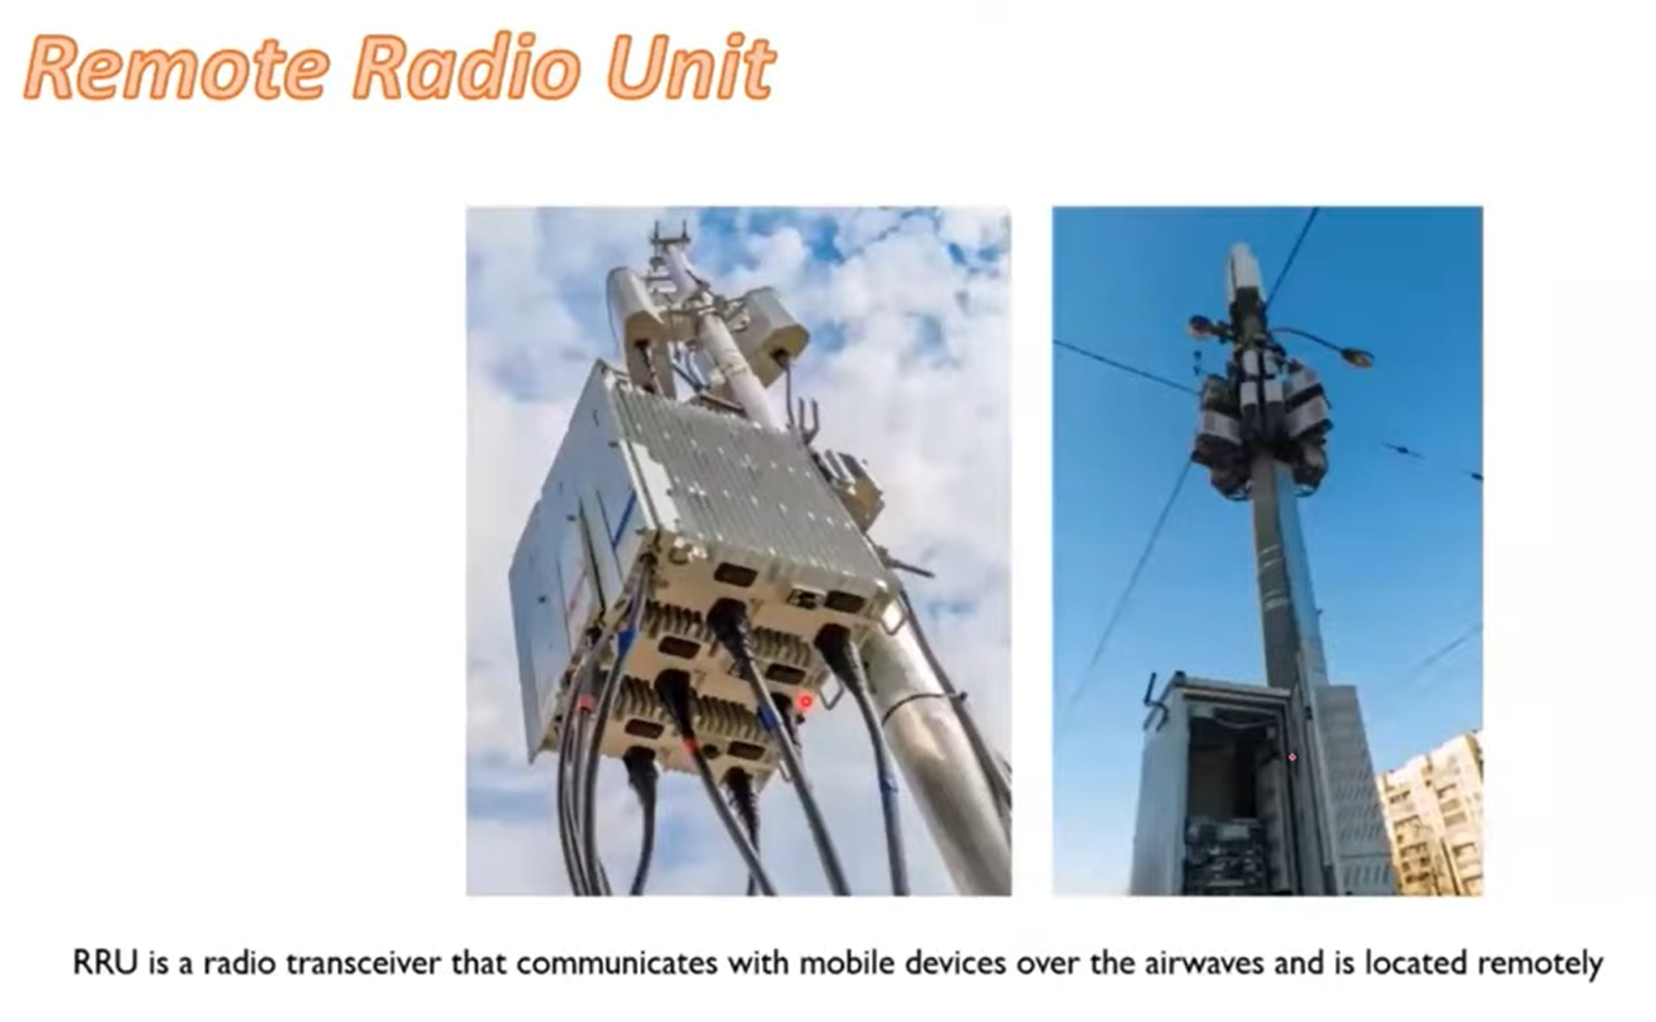
\includegraphics[width=.6\linewidth]{Pic/Remote_Radio_Unit}
	\caption{RRU}
	\label{fig:RRU}
\end{figure}

\begin{figure}[ht]
	\centering
	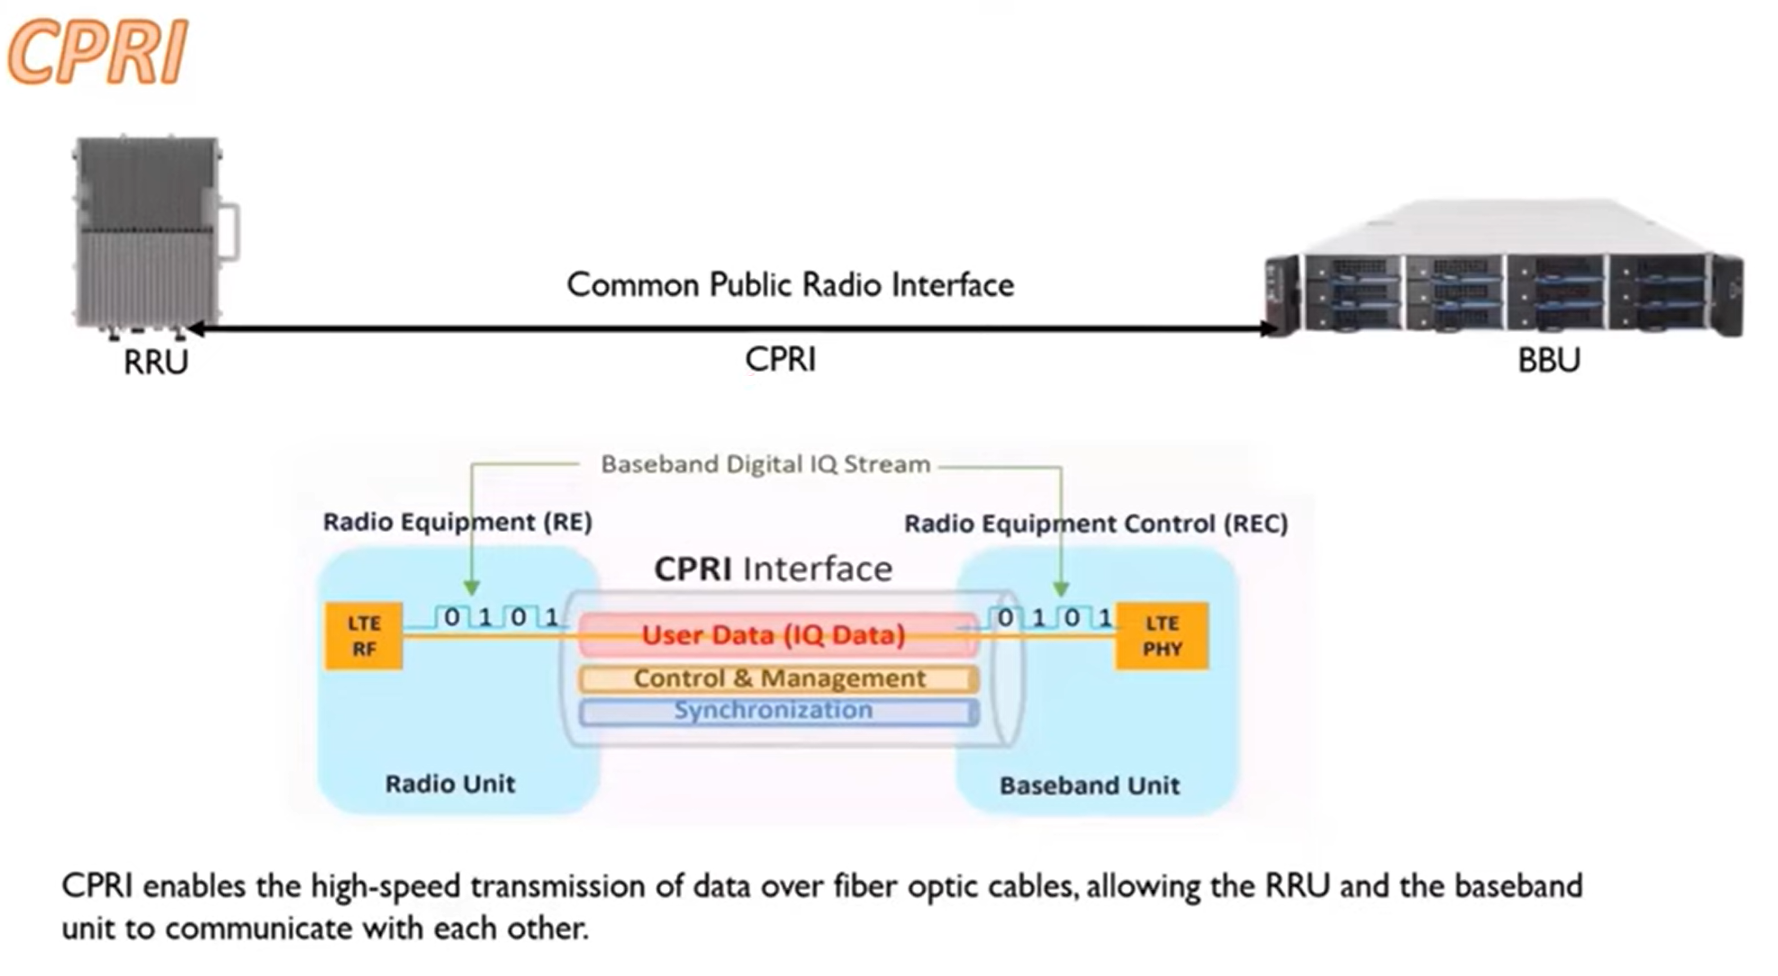
\includegraphics[width=.6\linewidth]{Pic/CPRI}
	\caption{CPRI}
	\label{fig:CPRI}
\end{figure}

در ناحیه
 \lr{RAN}
  به
   \lr{RRU}
    سخت افزار اختصاصی یا
     \lr{proprietary}
      می گویند و همچنین رابط میان
       \lr{RRU}
         و
          \lr{BBU}
           نیز اختصاصی و واحد
            \lr{BBU}
             خود شامل سخت افزار و نرم افزار اختصاصی است بدان معنا که اگر ما
              \lr{RRU}
               را از
                \lr{NOKIA}
                 خریداری کرده باشیم نمی‌توانیم
                  \lr{BBU}
                   را از
                    \lr{Ericsson}
                     خریداری کنیم.
                     
\chapter*{انواع 
RAN
}

\section*{CRAN}
به معنای
 \lr{Centralized RAN}
  است.
\section*{Virtual-RAN}                    
در حدود سال های 1994 ما دیوایس های مختلفی مثل رادیو،
 \lr{tape recorder}
 ، دوربین فیلم برداری،
  \lr{CD Player}
   و ... داشتیم و هم اکنون به کمک
    \lr{network function virtualization}
    گوشی همراه داریم و با کمک اپلیکیشن‌ها می‌توانیم عملکرد همان دستگاه ها را با کمک تلفن همراه داشته باشیم. به عبارتی ما به کمک
     \lr{NFV}
      ( 
    \lr{NETWORK FUNCTION VIRTUALIZATION} 
    ) از سخت افزار به نرم افزار گذر کردیم (شکل \ref{fig:vRAN})
    \begin{figure}[ht]
    	\centering
    	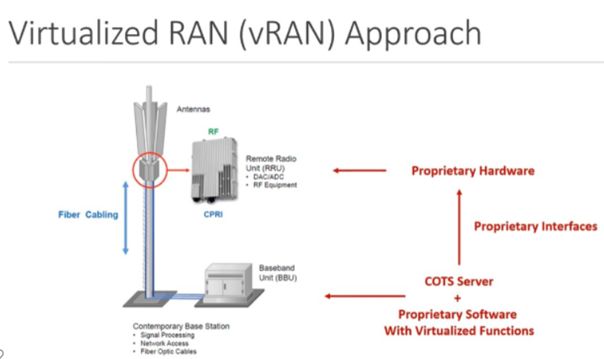
\includegraphics[width=.6\linewidth]{Pic/vRAN}
    	\caption{vRAN}
    	\label{fig:vRAN}
    \end{figure}
    
    
\section*{\lr{COTS (Commercial Of The Shells)}}
یک اصطلاح برای محصولات نرم افزاری است که قبلاً ساخته شده و برای خرید در دسترس هستند. در گذشته، برای گوش دادن به رادیو، شما نیاز داشتید یک دستگاه رادیو فیزیکی با آنتن و تیونر بخرید تا بتوانید ایستگاه‌های
 \lr{FM}
  یا
   \lr{AM}
    را دریافت کنید. این دستگاه به طور خاص برای این منظور طراحی شده بود و شما نمی‌توانستید از آن برای کاربردهای دیگر استفاده کنید. ما امروزه، شما می‌توانید به سادگی یک اپلیکیشن رادیو را روی گوشی هوشمند خود نصب کنید و با استفاده از اینترنت به ایستگاه‌های رادیویی گوش دهید. شما دیگر نیازی به خرید دستگاه فیزیکی خاصی ندارید، بلکه تنها با نصب یک نرم‌افزار روی یک سخت‌افزار چندمنظوره (گوشی هوشمند) می‌توانید به همان عملکرد دست پیدا کنید. در 
    \lr{Traditional RAN}
    ، برای پردازش سیگنال‌های رادیویی و مدیریت ارتباطات، نیاز به سخت‌افزارهای خاص و اختصاصی
    (
  \lr{proprietary hardware}
  ) مانند 
  \lr{Baseband Unit (BBU)}
   بود. این واحدها تنها برای این کار طراحی شده بودند و به راحتی قابل تغییر و تنظیم نبودند. در معماری
    \lr{vRAN}
     یا همان
      \lr{Virtual RAN}
     ، شما دیگر نیازی به استفاده از
      \lr{BBU}
      های اختصاصی (
       \lr{proprietary hardware}
    ) ندارید. به جای آن، می‌توانید از سرورهای استاندارد و تجاری (
    \lr{COTS}
    ) استفاده کنید. این سرورها چندمنظوره هستند و با نصب و پیکربندی  (
    \lr{Configuration}
    ) نرم‌افزارهای خاص، می‌توانند وظایف
     \lr{BBU}
     را انجام دهند. اما در
      \lr{Virtual RAN}
       همچنان یک چالش باقی می‌ماند: واحد
        \lr{RRU}
          و رابط میان آن با
           \lr{BBU}
            ، همچنان یک واحد اختصاصی (
            \lr{proprietary hardware}
            )باقی مانده است.در نتیجه نمیتوان واحد 
            \lr{RRU}
             را از یک
              \lr{Vendor}
              و  واحد 
              \lr{BBU}
               و 
               \lr{interface}
                 میان آن ‌هارا از دو
                  \lr{Vendor}
                   متفاوت تهیه کرد بدین معنا که اگر
                    \lr{BBU} 
                    از 
                    \lr{Ericsson}
                     خریداری شده،
                      \lr{RRU}
                       هم باید از
                        \lr{Ericsson}
                         خریداری شود. به این نکته توجه شود که
                          \lr{Virtual RAN}
                           همان
                            \lr{Open RAN}
                             نیست و در مسیر تکامل ناحیه دسترسی رادیو به
                              \lr{Open RAN}
                               قرار دارد.

در گذشته، هر تأمین‌کننده (
\lr{vendor}
) تجهیزات مخابراتی، سخت‌افزار و نرم‌افزارهای اختصاصی خود را برای اجرای وظایف مختلف شبکه ارائه می‌داد. این رویکرد مشکلاتی به همراه داشت. تجهیزات اختصاصی از چندین بخش و دستگاه مختلف تشکیل می‌شدند که فضای زیادی را اشغال می‌کردند و مصرف برق بالایی داشتند. هر دستگاه و بخش نیاز به رسیدگی فرد متخصص خود برای ارتقا و نگهداری داشت و این فرآیندها زمان‌بر و پرهزینه بودند و همچنین تغییرات و به‌روزرسانی سخت افزارهای‌ آن‌ها پیچیده بود که انعطاف‌پذیری شبکه را کاهش می‌داد. حال تغییر به سمت
 \lr{COTS}
 مزایای متعددی دارد که جلو تر به آن‌ها می‌پردازیم.

در
 \lr{Virtual RAN}
  بسیاری از وظایف مربوط به مدیریت و پردازش سیگنال‌های رادیویی از سخت‌افزارهای اختصاصی به سرورهای تجاری استاندارد (
  \lr{COTS}
  ) منتقل شدند. این تغییر به منظور کاهش هزینه‌ها، افزایش انعطاف‌پذیری و بهبود کارایی انجام می‌شود. با این حال، همچنان چالش‌هایی وجود دارد که منجر به حفظ وابستگی به تأمین‌کنندگان خاص (
  \lr{Vendor Lock-In}
  ) می‌شود. یکی از این چالش‌ها مربوط به رابط‌ها (
  \lr{interfaces}
  ) بین واحد  (
  \lr{BBU}
  ) و واحد (
  \lr{RRU}
  )  است.
  
  
  در قسمت بعد به بررسی 
  \lr{Open RAN}
  می پردازیم.
  
  \chapter*{OpenRAN}
  نیازمند به درک دو اصطلاح به نام
   GPP
    و
     SPP
      هستیم:
 \begin{enumerate}
 	\item پردازنده‌های عمومی (
 	{GPP}
 	)
 	\item پردازنده‌های خاص (
 	\lr{SPP}
 	)
 \end{enumerate}
 	\section*{پردازنده عمومی (
 		\lr{GPP - General Purpose Processor}
 		)}
 		
 	پردازنده‌های عمومی، همانطور که از نامشان پیداست، برای کاربردهای مختلف و متنوع طراحی شده‌اند. این پردازنده‌ها انعطاف‌پذیری بالایی دارند و می‌توانند با نصب و اجرای نرم‌افزارهای مختلف، وظایف متفاوتی را انجام دهند. یک دستگاه با پردازنده عمومی می‌تواند به عنوان
 	 \lr{MME (Mobility Management Entity)}
 	 ،
 	  \lr{AMF (Access and Mobility Management Function)}
 	  ،
 	   \lr{SGSN (Serving GPRS Support Node)}
 	    و غیره کار کند. تنها با نصب یا ارتقاء نرم‌افزار، می‌توان کارکرد آن را تغییر داد. با استفاده از پردازنده‌های عمومی که در حجم بالا تولید می‌شوند، هزینه‌ها کاهش می‌یابد. شرکت‌هایی مانند
 	     \lr{Intel (x86)}
 	     ،
 	      \lr{ARM}
 	      ،
 	       \lr{MIPS}
 	       ،
 	        \lr{SPARC} 
 	        و
 	         \lr{RISC-V}
 	         پردازنده‌های عمومی تولید می‌کنند که در بازارهای مختلفی استفاده می‌شوند. با توجه به اینکه پردازنده‌های عمومی در حجم بالا تولید و استفاده می‌شوند، تحقیقات و توسعه در این حوزه سریع‌تر صورت می‌گیرد و نوآوری با سرعت بیشتری اتفاق می‌افتد.
 	         
 	         
\section*{پردازنده خاص  (
	\lr{SPP - Specialized Purpose Processor}
	)}
	در 
	\lr{Traditional RAN}
	، از پردازنده‌های خاص استفاده می‌شد که برای یک وظیفه یا عملکرد خاص طراحی شده بودند. اگر یک دستگاه به عنوان 
	\lr{MME}
	 طراحی شده باشد، فقط می‌تواند به عنوان 
	 \lr{MME} 
	 عمل کند و نمی‌توان آن را برای کارکردهای دیگر استفاده کرد. این باعث محدودیت در استفاده می‌شود. پردازنده‌های خاص انعطاف‌پذیری کمتری دارند و برای تغییر کارکرد آن‌ها نیاز به تعویض سخت‌افزار وجود دارد که هزینه‌بر و زمان‌بر است. تولید و نگهداری پردازنده‌های خاص به دلیل محدود بودن کاربردهای آن‌ها و حجم تولید پایین‌تر، هزینه بیشتری دارد.
	 
	 
\section*{چرا 
	\lr{Open RAN}
	 ؟}
	در شبکه‌های دسترسی رادیویی سنتی (
	\lr{Traditional RAN}
	)، اپراتورهای شبکه با چندین چالش مواجه هستند.
	 \lr{Vendor lock-in}
	  یکی از این چالش هاست. وقتی یک واحد
	    \lr{baseband}
	    از یک فروشنده مثل اریکسون خریداری می‌شود، به اجبار بقیه تجهیزات مرتبط یعنی
	      \lr{RRU}
	      و
	       \lr{OSS}
	        هم باید از همان فروشنده تهیه شود. برای مثال، اگر شما یک
	         \lr{BBU} 
	         اریکسون (مدل‌هایی مانند 6630، 6651، 6648) داشته باشید، باید
	          \lr{RRU}
	          های اریکسون (مانند 4410، 4420، 2203، 4402، 4415) و
	           \lr{OSS}
	            اریکسون را هم تهیه کنید. امکان ترکیب تجهیزات از فروشندگان مختلف مثلاً
	             \lr{BBU}
	              از نوکیا،
	               \lr{RRU}
	                از اریکسون،
	                 \lr{OSS}
	                  از هواوی وجود ندارد زیرا رابط‌ها (
	                  \lr{interfaces}
	                  )  اختصاصی (
	                  \lr{proprietary hardware}
) و بسته هستند. چالش بعدی مربوط به هزینه های سرمایه ایست. بیشتر هزینه‌های سرمایه‌ای (
\lr{CapEx}
) برای ساخت یک شبکه بی‌سیم مربوط به بخش 
\lr{RAN}
 است و حدود 60-80 درصد از کل هزینه شبکه را شامل می‌شود. این هزینه بالا به دلیل نیاز به خرید یک مجموعه کامل تجهیزات از یک فروشنده است، بدون اینکه بتوان از گزینه‌های مقرون‌به‌صرفه‌تر از فروشندگان مختلف استفاده کرد. چالش دیگر کارایی عملیاتی پایین می‌باشد. وقتی رابط‌های نرم‌افزاری اختصاصی و به سخت‌افزار خاصی وابسته هستند، هرگونه به‌روزرسانی نرم‌افزاری به سخت‌افزار همان فروشنده وابسته خواهد بود. اگر اپراتور بخواهد فروشنده را تغییر دهد، باید تمام تجهیزات را عوض کند که این امر باعث می‌شود امکان تغییر تنها یک جزء از اجزای
  \lr{RAN}
   قدیمی وجود نداشته باشد.
   
	و اما مزایای 
	\lr{Open RAN}
	:
\begin{itemize}
\item \textbf{هوشمندی و مجازی سازی:}
به این معنا که می‌توان نرم‌افزارهای مختلف را روی سخت‌افزارهای استاندارد اجرا کرد. این امر به اپراتورها اجازه می‌دهد تا از تجهیزات متنوعی از فروشندگان مختلف استفاده کنند.
\item 
\textbf{قابلیت همکاری (
\lr{Interoperability}
): }
یکی از اصول کلیدی 
\lr{Open RAN}
 این است که
  \lr{BBU}
  ،
   \lr{RRU}
    و
     \lr{OSS}
      باید با رابط‌های باز
       (
       \lr{Open Interface}
       ) به هم متصل شوند. این قابلیت همکاری بین تجهیزات از فروشندگان مختلف امکان‌پذیر می‌سازد و باعث انعطاف‌پذیری بیشتر در انتخاب تجهیزات می‌شود.


\item \textbf{کاهش هزینه ها:} 
با استفاده از 
\lr{Open RAN}
، اپراتورها می‌توانند هزینه‌های
 \lr{CapEx}
  و
   \lr{OpEx}
    خود را کاهش دهند. از آنجا که امکان استفاده از تجهیزات مختلف از فروشندگان متعدد وجود دارد، اپراتورها می‌توانند گزینه‌های مقرون‌به‌صرفه‌تری را انتخاب کنند. همچنین، نیاز به تعویض کامل تجهیزات در صورت تغییر فروشنده از بین می‌رود، که این امر به کاهش هزینه‌ها و افزایش کارایی کمک می‌کند.

\end{itemize}
	به طور خلاصه،
	 \lr{Open RAN} 
	 با ارائه قابلیت همکاری، کاهش هزینه‌ها و افزایش انعطاف‌پذیری به اپراتورها اجازه می‌دهد تا شبکه‌های خود را به صورت کارآمدتر و مقرون‌به‌صرفه‌تر مدیریت کنند.
	
	در این نوع شبکه، تجهیزات بومی (
	\lr{COTS - Commercial Off-The-Shelf}
	) به جای تجهیزات خاص هر تولیدکننده استفاده می‌شوند. به این معنا که هر دو بخش
	 \lr{BBU (Baseband Unit)}
 و
   \lr{RRU (Remote Radio Unit)}
    و هم‌چنین
     \lr{interface} 
     بین آن‌ها نیز می‌توانند از سخت‌افزارهای بومی استفاده کنند.
	
	یکی از اصطلاحات کلیدی در این زمینه که در شکل \ref{fig:Open_RAN_Vision} نیز مشاهده می‎‌شود
	 \lr{SDR - Software Defined Radio}
	   است.
	    \lr{SDR}
	     را می‌توان از هر تولیدکننده اصلی طراحی
	      \lr{(ODM - Original Design Manufacturer)}
	       یا تولیدکننده تجهیزات اصلی 
	\lr{(OEM - Original Equipment Manufacturer)}
	 خریداری کرد. نکته مهم در 
	\lr{Open RAN}
	 این است که رابط بین
	  \lr{RRU}
	   و
	    \lr{BBU}
	     نیز باز (
	      \lr{Open Interface} 
	      ) است. این 
	بدین معنی است که می‌توان
	 \lr{RRU}
	 یک شرکت مانند
	  \lr{Nokia}
	   و
	    \lr{BBU}
	     یک شرکت دیگر مانند
	      \lr{Ericsson}
	        را با استفاده از این رابط باز به هم متصل کرد. در نتیجه مزیت بزرگ 
	        \lr{Open RAN}
	         این است که شما محدود به استفاده از تجهیزات و نرم‌افزارهای یک تولیدکننده خاص مانند
	          \lr{Nokia}
	          ، 
	         \lr{Ericsson}
	          یا
	           \lr{Huawei}
	          نیستید. بلکه می‌توانید تجهیزات و نرم‌افزارهای مختلف را از تولیدکنندگان مختلف خریداری و با هم ترکیب کنید که این امر انعطاف‌پذیری و تنوع بیشتری در شبکه به ارمغان می‌آورد. و هم‌چنین جهت بروز رسانی هر بخش نیازی به حضوری درسایت و تغییر
	           \lr{Config}
	            آن بخش نیست بلکه کافیست به صورت
	             \lr{remote}
	              ، نرم افزار روی آن را از نرم افزار دریافت شده از
	               \lr{Vendor A}
	                 به نرم افزار ذریافت شده از
	                  \lr{Vendor B}
	                    تغییر دهیم.
	
\begin{figure}[ht]
	\centering
	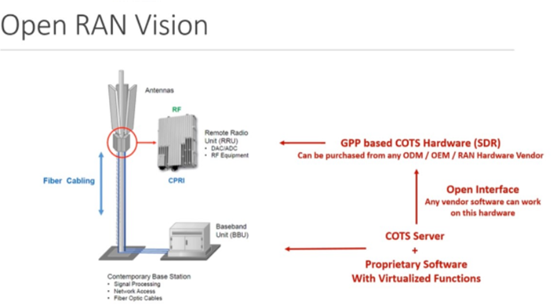
\includegraphics[width=.6\linewidth]{Pic/Open_RAN_Vision}
	\caption{\lr{Open RAN Vision}}
	\label{fig:Open_RAN_Vision}
\end{figure}

در
 \lr{V-RAN}
  طبق 
 تصویر \ref{fig:RAN_Area} به جای استفاده از سخت‌افزارهای اختصاصی، از یک محیط مجازی استفاده می‌شود. این بدان معناست که عملکردهای
  \lr{baseband (BBU)}
   می‌توانند بر روی سرورهای بومی (
   \lr{COTS}
   ) اجرا شوند. هرچند که
    \lr{BBU}
     می‌تواند بر روی سخت‌افزار بومی اجرا شود، ولی
      \lr{RRU}
       و رابط بین
        \lr{BBU}
         و
          \lr{RRU}
           هنوز هم بسته و اختصاصی هستند. این به معنای محدودیت در انتخاب تجهیزات و نرم‌افزارهای مختلف است.
در
 \lr{O-RAN}
  طبق تصویر \ref{fig:RAN_Area} نه تنها
   \lr{BBU}
    می‌تواند بر روی سخت‌افزار بومی اجرا شود، بلکه
     \lr{RRU}
      نیز می‌تواند از سخت‌افزار بومی استفاده کند. رابط بین
       \lr{BBU}
        و
         \lr{RRU}
          نیز باز است، که به معنای امکان استفاده از تجهیزات و نرم‌افزارهای مختلف از تولیدکنندگان متفاوت است.



\begin{figure}[ht]
	\centering
	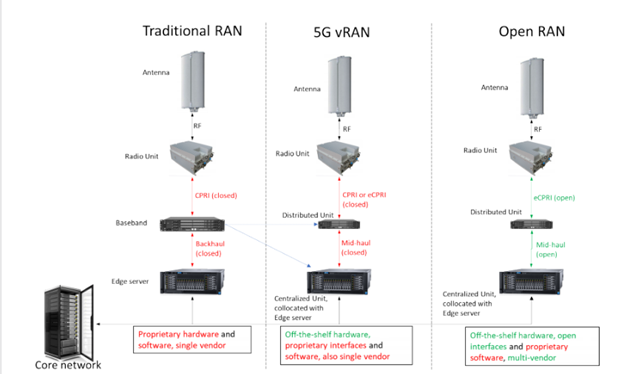
\includegraphics[width=.6\linewidth]{Pic/RAN_Area}
	\caption{تفاوت ناحیه 
		\lr{RAN}
		  در ۳ حالت
		   \lr{Traditional}
		   ،
		    \lr{Virtual}
		      و
		       \lr{Open RAN}
		        }
	\label{fig:RAN_Area}
\end{figure}


\section*{
\lr{RAN}
و
\lr{OSI}
هفت لایه
}
برای درک بهتر معماری
 \lr{Open RAN}
 ، می‌توانیم اجزای مختلف
  \lr{RAN}
   را با لایه‌های مدل
    \lr{OSI (Open Systems Interconnection)}
    تطبیق دهیم. مدل
     \lr{OSI}
      یک مدل هفت‌لایه‌ای برای استانداردسازی عملکرد شبکه‌ها است (شکل \ref{fig:OSI7Layer}).
      \lr{RRU}
      در لایه فیزیکی (
      \lr{Physical Layer}
      ) مدل
       \lr{OSI}
        قرار می‌گیرد. وظایف اصلی
         \lr{RRU}
         شامل:
\begin{itemize}
\item
\textbf{ تبدیل
  \lr{RF} 
  (
  \lr{RF Conversion}
  )
  :}
تبدیل سیگنال‌های رادیویی به سیگنال‌های دیجیتال و برعکس (تبدیل آنالوگ به دیجیتال و دیجیتال به آنالوگ).
\item 
\textbf{تبدیل‌های
 \lr{RF}
  (
  \lr{RF Transformations}
  ): }
وظایفی مانند تقویت سیگنال، فیلترگذاری و تبدیل فرکانس‌ها نیز در این لایه انجام می‌شود.
\item 
\textbf{مدولاسیون و دمدولاسیون
  (
  \lr{Modulation and Demodulation}
  ):}
تغییر سیگنال‌ها برای انتقال داده‌ها. 
\end{itemize}
     \begin{figure}[ht]
     	\centering
     	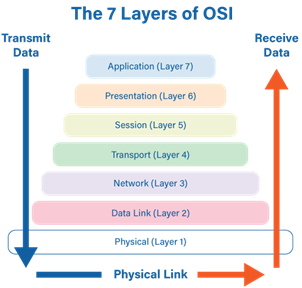
\includegraphics[height=.3\linewidth]{Pic/OSI7Layer}
     	\caption{هفت لایه
     		\lr{OSI}
     	}
     	\label{fig:OSI7Layer}
     \end{figure}
     
     
      \lr{BBU}
        مسئول اجرای پروتکل‌های مختلف و وظایف پیشرفته‌تر در لایه‌های بالاتر از لایه فیزیکی است. پروتکل‌ها و وظایف BBU شامل:
\begin{itemize}
\item
\textbf{\lr{RRC (Radio Resource Control)}
:}
این پروتکل در لایه شبکه (
\lr{Network Layer}
) قرار می‌گیرد و مسئولیت مدیریت ارتباطات، پخش و ارسال پیام‌ها، مدیریت ارتباط و تحرک (
\lr{mobility}
) و گزارش‌دهی را بر عهده دارد.
\item
 \textbf{\lr{PDCP (Packet Data Convergence Protocol)}
 :}
 این پروتکل در لایه شبکه (
 \lr{Network Layer}
 ) قرار دارد و وظایفی مانند مدیریت
  \lr{header}
   های
     \lr{IP}
     ، امنیت و عملکردهای دیگری مانند رمزنگاری (
     \lr{ciphering}
     ) و حفاظت یکپارچگی (
     \lr{integrity protection}
     ) را انجام می‌دهد.
\item
\textbf{\lr{RLC (Radio Link Control)}
:}
این پروتکل در لایه پیوند داده (
\lr{Data Link Layer}
) قرار می‌گیرد و مسئولیت‌هایی مانند تکه‌تکه کردن (
\lr{segmentation}
) و بازترکیب  (
\lr{reassembly}
) داده‌ها، کنترل جریان و تصحیح خطا را بر عهده دارد.
\item
\textbf{\lr{MAC (Medium Access Control)}
:}
 این لایه نیز در لایه پیوند داده (
 \lr{Data Link Layer}
 ) قرار می‌گیرد و وظایفی مانند دسترسی به رسانه، تجمع حامل (
 \lr{carrier aggregation}
 )، نگاشت کانال‌ها
  \lr{HARQ (Hybrid Automatic Repeat Request)}
   و زمان‌بندی بسته‌ها را بر عهده دارد.
\item
\textbf{\lr{PHY (Physical Layer)}
:}
این لایه شامل تمامی وظایف اصلی لایه فیزیکی مانند کدگذاری و دکدگذاری (
\lr{Coding and Decoding}
)، مدولاسیون و دمدولاسیون (
 \lr{Modulation and Demodulation}
 )، مدیریت منابع و اجرای
  \lr{IFFT/FFT} 
  (تبدیل فوریه و تبدیل فوریه معکوس) است.
\end{itemize}

      
\chapter*{تقسیم واحدهای رادیویی، مرکزی و توزیع شده}   
در شبکه‌های نسل ۵ ، مفهومی به نام "
\lr{RU / CU / DU Split}
" یا "تقسیم واحدهای رادیویی، مرکزی و توزیع شده" وجود دارد که نقش مهمی در بهبود کارایی و انعطاف‌پذیری شبکه دارد (شکل \ref{fig:RU_CU_DU_Splits}).

در معماری شبکه های نسل چهار، سه عنصر اصلی داشتیم که هسته شبکه،
 \lr{BBU}
  و
   \lr{RRU}
    بودند و ارتباط میان هسته شبکه با
     \lr{BBU}
      از طریق
       \lr{Backhaul}
        و ارتباط میان
         \lr{BBU} 
         و
          \lr{RRU} 
          از طریق
           \lr{Fronthaul}
            بود  واحد پردازش پایه‌ای
             (
             \lr{BBU}
             ) یک موجودیت تکی است که مسئول پردازش هم پروتکل‌های لایه‌های بالاتر و هم سیگنال‌های لایه‌های پایین است. 
حال به معماری شبکه های نسل پنج و مفهوم
 \lr{Split}
  می پردازیم، در این نسل برای افزایش انعطاف‌پذیری و مقیاس‌پذیری، معماری شبکه بهینه‌سازی شده و بخش
  \lr‌{Baseband}
   به دو واحد مجزا تقسیم شده‌است. عملکرد  واحد
    \lr{BBU}
     به ۲ مولفه جداگانه محول می‌شود.
\begin{itemize}
	\item 
	\textbf{واحد مرکزی (
	\lr{CU - Centralized Unit}
	):}
	مسئول مدیریت پروتکل‌های لایه بالاتر و برخی از وظایف شبکه‌ای است.
	\item 
\textbf{واحد توزیع شده (
	\lr{DU - Distributed Unit}
	):}
	وظایف پردازش سیگنال‌های لایه پایین و ارتباطات محلی را بر عهده دارد.
\end{itemize}
این تقسیم‌بندی که تحت استاندارد
 \lr{3GPP	TR 38.801}
  معرفی شده است، به نام "
  \lr{Network Split}
  " یا
"
\lr{RU / CU / DU Split}
" شناخته می‌شود.
یکی از مزایای این نوع
 \lr{Split}
 ،
  \lr{Cloud Optimization} 
  است. با استفاده از معماری تقسیم‌بندی شده، وظایف پردازش می‌تواند به صورت مجازی بر روی سرورهای ابری اجرا شوند که این امر باعث کاهش هزینه‌ها و افزایش کارایی می‌شود.

\begin{figure}[ht]
	\centering
	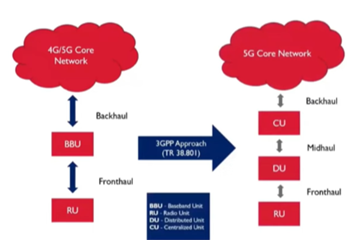
\includegraphics[width=.6\linewidth]{Pic/RU_CU_DU_Splits}
	\caption{\lr{RU / CU / DU Splits}}
	\label{fig:RU_CU_DU_Splits}
\end{figure}

\subsection*{
	\lr{Midhaul}
	 (
	  رابط میانی
	   \lr{CU}
	    و
	     \lr{DU}
	  ) :}
	  
این رابط وصل‌کننده واحدهای
 \lr{CU}
  و
   \lr{DU}
    است. این رابط تبادل داده و سیگنال‌های کنترلی بین این دو مولفه را فراهم می‌کند. رابط میانی امکان هماهنگی و همگام‌سازی بین عناصر پردازش مرکزی و توزیع شده را  نیز فراهم می‌کند.
    
\begin{figure}[ht]
   	\centering
   	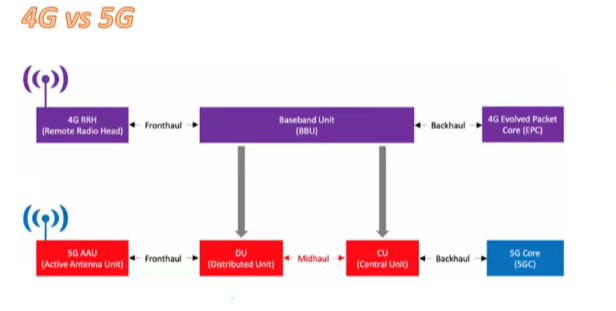
\includegraphics[width=.6\linewidth]{Pic/4G_5G}
   	\caption{مقایسه نسل چهار و نسل پنج
   	}
   	\label{fig:4G_5G}
\end{figure}

\begin{figure}[ht]
   	\centering
   	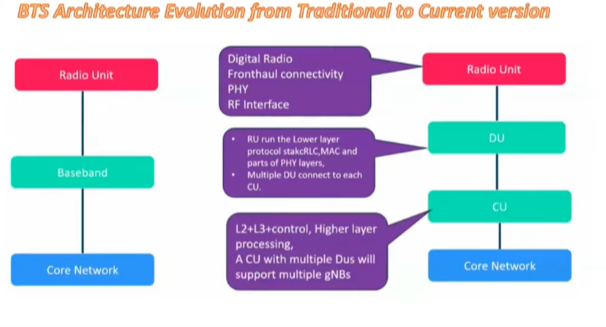
\includegraphics[width=.6\linewidth]{Pic/BTS_Evaluation}
   	\caption{تکامل معماری
   		\lr{BTS}    		از گذشته تا ورژن کنونی
    	}
   	\label{fig:BTS_Evaluation}
\end{figure}
\subsection*{وظایف هر کدام از واحدها در نسل ۵:}
\subsubsection*{واحد
	 \lr{RU}
	 }
\textbf{پردازش دیجیتال مقدماتی یا
 \lr{DFP ( Digital Front End)} 
 :} 
مسئول انجام پردازش‌های دیجیتال اولیه بر روی سیگنال‌هاست. این پردازش‌ها شامل تقویت سیگنال، تبدیل فرکانس و فیلترگذاری است.بخشی از پروتکل های لایه فیزیکال را نیز مدیریت می‌کند.
\subsubsection*{واحد
	 \lr{DU}}
پروتکل‌های لایه
 \lr{RLC}
، لایه
 \lr{MAC}
  و بخش‌هایی از لایه فیزیکی بسته به نوع تقسیم عملکرد را اجرا می‌کند. چندین
   \lr{DU}
    به یک
     \lr{CU}
      متصل می‌شوند.
\subsubsection*{واحد 
	\lr{CU}}
به دلیل آنکه چندین
 \lr{DU}
  به یک
   \lr{CU}
    متصل می‌شوند،
     \lr{CU}
      وظیفه دارد عملیات چندین
       \lr{DU}
        را کنترل ‌کند. به همین دلیل، در بسیاری از موارد،
         \lr{DU}
          با
           \lr{RU}
            در محل قرار می‌گیرد تا وظایف سنگین مانند
             \lr{FFT}
              و
               \lr{IFFT}
                را انجام دهد و تأخیر کم داشته باشد. این واحد پروتکل هایی مانند
                 \lr{RRC}
                  و لایه
                   \lr{PDCP}
                    را اجرا می‌کند.
                    
حال ۲ نوع اتصال میان
 \lr{CU}
  و
   \lr{DU}
    وجود دارد :
اگر این اتصال از نوع
 \lr{Control Plane}
  باشد به آن
   \lr{F1c}
    و اگر از نوع
     \lr{User Plane}
      باشد به آن
       \lr{F1u}
        گویند.
        
 \section*{مفهوم 
 	\lr{Edge Computing}
 	}
در شبکه‌های 5G، مفهوم مهمی به نام "
\lr{Edge Computing}
" وجود دارد که به معنای انجام پردازش و ذخیره‌سازی داده‌ها و برنامه‌ها در نزدیکی منابع محاسباتی و ذخیره‌سازی کاربران است. در این حالت، پردازش و ذخیره‌سازی داده‌ها به صورت محلی و در محدوده نزدیک به کاربران انجام می‌شود، به جای انتقال تمام داده‌ها به مراکز داده ابری ( 
\lr{Cloud Data Center} 
) دورتر.

برای امکان‌سنجی
 \lr{Edge Computing}
  در شبکه‌های
   \lr{5G}
   ، نیاز به تقسیم وظایف بین واحدهای مرکزی (
   \lr{Distributed Unit - DU}
   ) و واحدهای مرکزی (
	 \lr{Centralized Unit - CU}
	 ) وجود دارد. با این تقسیم بندی، پردازش و تصمیم‌گیری‌های محاسباتی می‌توانند به صورت محلی و در نزدیکی منابع فیزیکی انجام شود، که منجر به بهبود عملکرد شبکه و ارائه سرویس‌های با کیفیت واقعی زمانی (
	 \lr{Real-Time}
	 ) می‌شود.
	 
\section*{
	هدف از جداسازی
	 \lr{DU} 
	 از
	  \lr{RU}
	   در معماری شبکه 
	   \lr{5G}
	    }	 
چند دلیل برای جداسازی واحد توزیع (
\lr{DU}
) از واحد رادیویی (
\lr{RU}
) در شبکه‌های
 \lr{5G}
  وجود دارد:
  \begin{enumerate}
  	\item
  	\textbf{کاهش هزینه:}
  	 یک واحد رادیویی ساده‌تر که توان پردازشی کمتری دارد، ارزان‌تر ساخته می‌شود. هوشمندی و قدرت پردازش در واحد توزیع متمرکز شده که با استفاده از فناوری‌های پیشرفته مانند هوش مصنوعی، یادگیری ماشین و رایانش ابری (
  	 \lr{Cloud Computing}
  	 )، کارآمدتر اجرا می‌شود. این کار باعث کاهش هزینه کل سخت‌افزار  ساختار شبکه می‌شود.
  	\item
  	\textbf{مدیریت بهتر منابع:}
  	با جداسازی واحد توزیع، می‌توانیم گروهی از واحدهای رادیویی را به طور همزمان مشاهده و مدیریت کنیم که تصویر وسیع‌تری از شبکه به ما می‌دهد. این امکان را برای ویژگی‌هایی مانند توازن بارگذاری چند نقطه‌ای هماهنگ (
  	\lr{Comp}
  	) فراهم می‌کند.
  	\lr{Comp}
  	می‌تواند به طور پویا بار کاری را در بین چندین واحد رادیویی توزیع کند و بدین ترتیب استفاده از منابع را بهینه کرده و عملکرد شبکه را بهبود بخشد.
  	\item 
  	\textbf{طراحی انعطاف‌پذیر شبکه:} 
  	معماری توزیع‌شده به توزیع انعطاف‌پذیرتر وظایف پردازشی بین واحد مرکزی (
  	\lr{CU}
  	) و واحد توزیع (
  	\lr{DU}
  	) امکان می‌دهد. این انعطاف‌پذیری به طراحان شبکه اجازه می‌دهد تا شبکه را بر اساس عوامل مختلفی شبکه را با سناریوهای استقرار متنوع سازگار سازد.
  \end{enumerate}

\begin{figure}[ht]
	\centering
	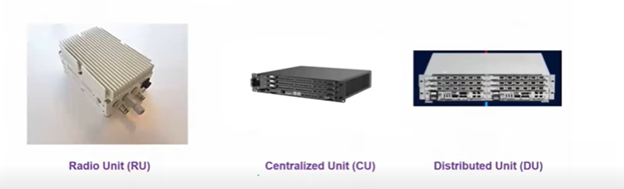
\includegraphics[width=.6\linewidth]{Pic/RU_CU_DU}
	\caption{
		\lr{RU}    		
		،
		\lr{CU}
		و 
		\lr{DU}
	}
	\label{fig:RU_CU_DU}
\end{figure}
 
 \subsection*{ انعطاف‌پذیری در محل استقرار لایه‌های پروتکل در شبکه دسترسی رادیویی
 	\lr{5G(RAN)}}
 در شبکه‌های 
 \lr{5G}
 ، برخلاف نسل‌های قبلی که تمام پردازش‌ها در یک واحد انجام می‌شد، امکان تقسیم این واحد ( 
 \lr{gNodeB}
 )
  به دو بخش مرکزی (
  \lr{CU}
  ) و توزیع‌شده (
  \lr{DU}
  ) وجود دارد. نکته‌ی کلیدی در این معماری توزیع‌شده، انعطاف‌پذیری در محل استقرار لایه‌های مختلف پروتکل است.
 
 \subsection*{عوامل تعیین‌کننده‌ی محل استقرار لایه‌های پروتکل:}
 \begin{itemize}
\item 
\textbf{قابلیت‌های تامین‌کننده(
Vendor
):} شرکت‌های مختلف ممکن است گزینه‌های مختلفی برای محل استقرار لایه‌های پروتکل ارائه دهند.
\item 
\textbf{اولویت اپراتور:} اپراتورهای شبکه می‌توانند بر اساس نیازهای خود، محل استقرار لایه‌ها را انتخاب کنند.
 \end{itemize}
 
\subsection*{مثال:
	 \lr{Option 2}}
فرض کنید از گزینه تقسیم ۲ طبق شکل \ref{fig:Functional_Split_Options_for_5G} استفاده می‌کنیم. در این حالت:
\begin{itemize}
	\item 
	\textbf{واحد مرکزی (
	\lr{CU}
	): }
	شامل لایه‌های
	 \lr{PDCP}
	   و
	    \lr{RRC}
	      می‌شود. این لایه‌های سطح بالا مسئولیت رمزنگاری داده، سیگنالینگ کنترل و تخصیص منابع را بر عهده دارند.
	\item 
\textbf{واحد توزیع‌شده (
	\lr{DU}
	):}
	 شامل پروتکل‌های
	  \lr{High RLC}
	   ،
	    \lr{Low RLC}
	    ،
	     \lr{High MAC}
	     ،
	      \lr{Low MAC}
	      و    
	\lr{High PHYSICAL}
	 است. این لایه‌ها وظایف بخش‌بندی داده، کنترل خطا و انتقال لایه فیزیکی را انجام می‌دهند.
	
	\item 
	\textbf{واحد رادیویی (
	RU
	):}
	 شامل قابلیت‌های
	  \lr{RF}
	   و
	    \lr{Low Physical}
	      است. این بخش مسئول تبدیل سیگنال رادیویی و فرآیندهای اولیه‌ی ارسال و دریافت است.
\end{itemize}

\begin{figure}[ht]
	\centering
	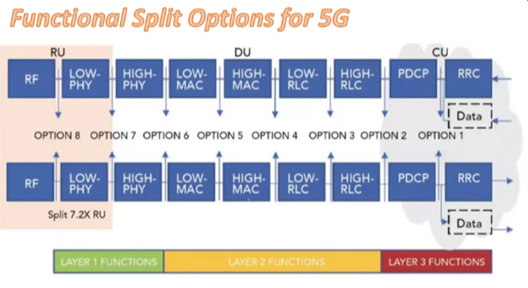
\includegraphics[width=.6\linewidth]{Pic/Functional_Split_Options_for_5G}
	\caption{گزینه های
		\lr{5G}    		
	}
	\label{fig:Functional_Split_Options_for_5G}
\end{figure}


\chapter*{سه مورد سناریو کاربردی در معماری نسل پنج}
 \section*{
 	باند پهن همراه پیشرفته (
 	\lr{eMBB - Enhanced Mobile Broadband}
 	):}
 	\begin{itemize}
 		\item \textbf{نیاز:}
ارائه نرخ داده بالا برای برنامه‌هایی مانند استریم ویدیوی با وضوح بالا، بازی‌های ابری (
\lr{Cloud Gaming}
) و دانلود سریع فایل‌ها.
 		\item \textbf{مشخصات:}
 		\begin{itemize}
 			\item 
 نیاز به پهنای باند زیاد و ظرفیت بالا در شبکه.
 			\item 
استفاده از تکنیک‌هایی مانند
 \lr{MIMO (Multiple-Input Multiple-Output)}
 و فرکانس‌های بالا برای افزایش سرعت داده.
 			\item 
 مناسب برای مناطق پرجمعیت و برنامه‌های پرمصرف داده.
 		\end{itemize}
 	\end{itemize}
 	
 	\section*{
 	ارتباطات فوق قابل اعتماد با تأخیر کم 
 	\lr{(URLLC - Ultra-Reliable Low-Latency Communication)}
 	:}
 	\begin{itemize}
 		\item \textbf{نیاز:}
 		ارائه ارتباطات با تأخیر بسیار کم و قابل اعتماد برای برنامه‌هایی مانند جراحی از راه دور، کنترل خودروهای خودران و اینترنت اشیا صنعتی.
 		\item \textbf{مشخصات:}
 		\begin{itemize}
 			\item 
نیاز به تأخیر بسیار کم (زیر 1 میلی‌ثانیه) و قابلیت اطمینان بالا.
 			\item 
 استفاده از تکنیک‌هایی مانند برش شبکه (
 \lr{Network Slicing}
 ) و تخصیص اختصاصی منابع برای تضمین کیفیت خدمات.
 			\item 
 	مناسب برای برنامه‌هایی که به زمان‌بندی دقیق و قابلیت اطمینان حیاتی نیاز دارند.
 		\end{itemize}
 	\end{itemize}
 	
 	\section*{
 		ارتباطات گسترده نوع ماشین
 		 \lr{(mMTC - Massive Machine Type Communication)}
 		 :}
 	\begin{itemize}
 		\item \textbf{نیاز:}
 		اتصال تعداد زیادی از دستگاه‌های کم‌مصرف با ترافیک داده کم، مانند سنسورها، مترها و ردیاب‌ها.
 		\item \textbf{مشخصات:}
 		\begin{itemize}
 			\item 
 	نیاز به اتصالات کارآمد و مقرون به صرفه برای تعداد زیادی از دستگاه‌ها.
 			\item 
 	استفاده از تکنیک‌هایی مانند
 	 \lr{LPWA}
 	  (شبکه‌های با توان کم و برد گسترده) برای افزایش عمر باتری و کاهش هزینه‌ها.
 			\item 
 			مناسب برای برنامه‌های اینترنت اشیا (
 			\lr{IoT}
 			) که در آن حجم زیادی از داده‌های حسگر با سرعت کم جمع‌آوری می‌شود
 		\end{itemize}
 	\end{itemize}
 	
 	
\chapter*{تقسیم بندی درون CU}
طبق شکل \ref{fig:Logical_RAN_Disaggregation}
 \lr{CU}
 را می‌توان به دو زیربخش دیگر تقسیم کرد:
\begin{itemize}
	\item 
	\textbf{صفحه‌ی کنترل (
	\lr{CP – Control Plane}
	):}
	 مدیریت سیگنالینگ شبکه و توابع کنترل را انجام می‌دهد.
	\item 
	\textbf{صفحه‌ی کاربر (
	\lr{UP - UserPlane}
	): }
	پردازش داده‌های کاربر و تخصیص منابع را مدیریت می‌کند.
\end{itemize}
\section*{چالش تاثیر فاصله بر تاخیر: }
فاصله فیزیکی بین کاربر و
\lr{BBU}
(که اکنون به
\lr{CU}
و
\lr{DU}
تقسیم شده است) باعث ایجاد تأخیر می‌شود. این تأخیر می‌تواند برای برنامه‌هایی که نیازمند ارتباطات فوق قابل اعتماد با تأخیر کم (
\lr{URLLC}
) هستند، چالش‌برانگیز باشد.
\begin{figure}[ht]
	\centering
	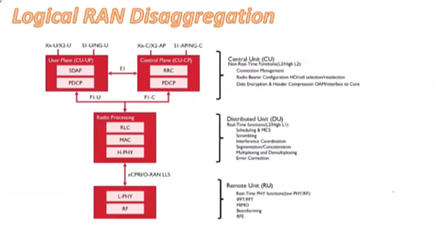
\includegraphics[width=.6\linewidth]{Pic/Logical_RAN_Disaggregation}
	\caption{
		تفکیک
		\lr{Logical RAN}
	}
	\label{fig:Logical_RAN_Disaggregation}
\end{figure}

\section*{مقابله با چالش‌های تأخیر در
	  \lr{URLLC}
	   }
برای دستیابی به
 \lr{URLLC}
 با وجودِ احتمال دور بودنِ شبکه‌ی مرکزی، معماری توزیع‌شده به روش زیر کمک می‌کند:
 \subsection*{نزدیک کردن پردازش به کاربران:}
با قرار دادن واحد رادیویی (
\lr{RU}
) با قابلیت‌های
 \lr{Low Physical Layer}
   و
    \lr{RF}
     نزدیک به کاربر، پردازش اولیه‌ی سیگنال نزدیک‌تر به منبع رخ می‌دهد. این کار باعث کاهش مسافتی می‌شود که نور برای پردازش اولیه نیاز دارد و در نتیجه تأخیر را به حداقل می‌رساند.
     
     
 در شبکه
  \lr{5G}
   سه رابط وجود دارد (شکل \ref{fig:Fronthaul_Midhaul_Backhaul}):
   \begin{itemize}
   	\item \textbf{\lr{Fronthaul}:}
   	  بین واحد توزیع‌شده (
   	  \lr{DU}
   	  ) و واحد رادیویی (
   	  \lr{RRU}
   	  )
   	\item \textbf{\lr{Midhaul}:}
   	بین واحد مرکزی (
   	\lr{CU}
   	) و واحد توزیع‌شده (
   	\lr{DU}
   	)
   	\item \textbf{\lr{Backhaul}:}
   	بین واحد مرکزی (
   	\lr{CU}
   	) و هسته‌ی شبکه
   \end{itemize}
     
\begin{figure}[ht]
	\centering
	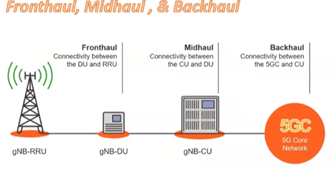
\includegraphics[width=.6\linewidth]{Pic/Fronthaul_Midhaul_Backhaul}
	\caption{ روابط
		\lr{Fronthaul}    		
		،
		\lr{Midhaul}
		و 
		\lr{Backhaul}
		در شبکه
		\lr{5G}
	}
	\label{fig:Fronthaul_Midhaul_Backhaul}
\end{figure}

\begin{figure}[ht]
	\centering
	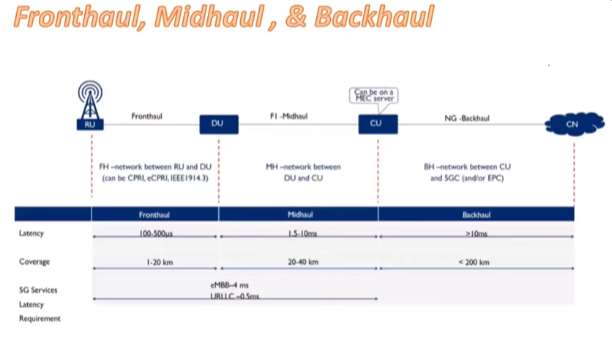
\includegraphics[width=.6\linewidth]{Pic/DUI}
	\caption{  \r{(DU)} و   \r{(CU)}  در فاصله ۲۰ تا ۴۰ کیلومتر
	}
	\label{fig:Fronthaul_Midhaul_Backhaul}
\end{figure}

تقسیم‌بندی \lr{RAN} در شبکه‌های نسل ۵ به اپراتورها این امکان را می‌دهد تا شبکه را بر اساس نیازهای خاص هر منطقه و سرویس، بهینه کنند. در اینجا سه عامل کلیدی در این فرایند آورده شده است:

\section*{ نیاز به پشتیبانی از کیفیت خدمات خاص (\lr{QoS – Quality of Service}) برای سرویس‌های مختلف (کیفیت خدمات به معنای سطح تضمین شده‌ی عملکرد برای یک سرویس است):}

\begin{itemize}
    \item شبکه‌های ۵G انواع مختلفی از سرویس‌ها را ارائه می‌دهند، از جمله:
    \begin{itemize}
        \item باند پهن همراه پیشرفته (\lr{eMBB})
        \item ارتباطات فوق قابل اعتماد با تأخیر کم (\lr{URLLC})
        \item ارتباطات گسترده نوع ماشین (\lr{mMTC})
    \end{itemize}
    \item هر یک از این سرویس‌ها به سطح متفاوتی از کیفیت خدمات (\lr{QoS}) نیاز دارند. برای مثال، \lr{URLLC} نیازمند تأخیر بسیار پایین است، در حالی که \lr{eMBB} بیشتر به نرخ داده بالا اهمیت می‌دهد. با تقسیم‌بندی \lr{RAN}، اپراتورها می‌توانند پردازش‌های مربوط به هر سرویس را به بخش‌های مختلف شبکه اختصاص دهند.
\end{itemize}

\section*{پشتیبانی از تراکم کاربر و تقاضای بار خاص در هر منطقه جغرافیایی (حجم و میزان ترافیک استفاده از شبکه):}

\begin{itemize}
    \item تراکم کاربر در مناطق مختلف شبکه متفاوت است. در مناطق پرجمعیت، تعداد کاربران بیشتر و تقاضای بار شبکه (ترافیک) بالاتر است، در حالی که در مناطق کم‌جمعیت کاربران کمتری وجود دارد.
    \item تقسیم‌بندی \lr{RAN} به اپراتورها این امکان را می‌دهد تا منابع شبکه را بر اساس تقاضای مناطق مختلف تخصیص دهند. در مناطق پرجمعیت، می‌توان از \lr{CU} و \lr{DU} با ظرفیت بالا استفاده کرد، در حالی که در مناطق کم‌جمعیت می‌توان از واحدهای با ظرفیت پایین‌تر استفاده کرد.
    \item این امر باعث می‌شود تا استفاده از منابع شبکه بهینه شود و هزینه‌ی راه‌اندازی و نگهداری کاهش یابد.
\end{itemize}

\section*{در دسترس بودن شبکه‌های انتقال با سطوح کارایی مختلف (شبکه انتقال، شبکه‌ای است که وظیفه‌ی انتقال داده‌ها بین بخش‌های مختلف شبکه را برعهده دارد):}

\begin{itemize}
    \item هزینه‌های مربوط به راه‌اندازی و نگهداری شبکه‌های انتقال، به ویژه فیبر نوری، بالا است.
    \item در تقسیم‌بندی \lr{RAN}، اپراتورها می‌توانند نوع و ظرفیت شبکه انتقال را بر اساس نیازهای سرویس و تراکم کاربر در هر منطقه انتخاب کنند.
    \item برای مثال، در مناطق پرجمعیت که نیازمند ظرفیت بالا و نرخ داده زیاد هستند، از شبکه‌های انتقال پرظرفیت مانند فیبر نوری استفاده می‌شود. در مناطق کم‌جمعیت، می‌توان از شبکه‌های انتقال با ظرفیت پایین‌تر مانند مایکروویو استفاده کرد که هزینه‌ی کمتری دارند.
    \item با انتخاب مناسب شبکه‌ی انتقال، می‌توان هزینه‌ها را به حداقل رساند و در عین حال عملکرد مطلوبی را برای کاربران در مناطق مختلف شبکه تضمین کرد.
\end{itemize}

\begin{figure}[ht]
	\centering
	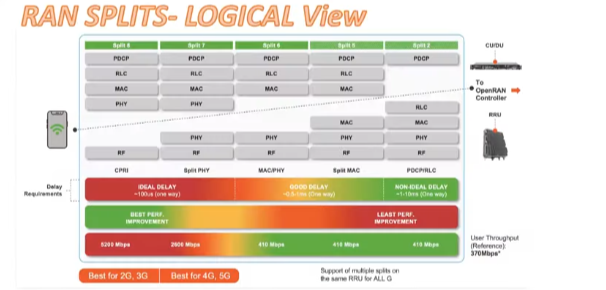
\includegraphics[width=.6\linewidth]{Pic/RAN}
	\caption{  مقایسه \r{Option7} و \r{Option8}
	}
	\label{fig:Fronthaul_Midhaul_Backhaul}
\end{figure}
\section*{
تقسیم‌بندی شبکه دسترسی رادیویی 
\r{(RAN)}
 در
 \r{Open RAN}
}
چرا \lr{Split 7} برای نسل ۴ و ۵ و \lr{Split 8} برای نسل ۲ و ۳ توصیه می‌شود؟
مقایسه \lr{Option 7} و \lr{Option 8}:

\subsection*{\lr{Option 7} :}
بیشتر پردازش‌ها (\lr{PDCP}، \lr{RLC}، \lr{MAC}، \lr{High Physical layer}) را در \lr{DU} قرار می‌دهد و فقط توابع \lr{RF} و لایه فیزیکی پایین در واحد رادیویی (\lr{RU}) باقی می‌مانند. این گزینه به دلیل موارد زیر برای شبکه‌های نسل ۴ و نسل ۵ ایده‌آل است:
\begin{itemize}
    \item انعطاف‌پذیری: بر اساس تقاضای متفاوت کاربران و انواع سرویس‌ها \lr{eMBB}، \lr{URLLC}، \lr{mMTC} امکان تغییر مستقل قدرت پردازش در \lr{CU} و \lr{DU} را فراهم می‌کند.
    \item کاهش پهنای باند \lr{Fronthaul}: با انتقال بار پردازشی به \lr{DU}، داده‌هایی که پیچیدگی کمتری دارند بین \lr{DU} و \lr{RU} نیاز به جابه‌جایی دارند که در نتیجه، نیاز به پهنای باند \lr{Fronthaul} را کاهش می‌دهد.
\end{itemize}

\subsection*{\lr{Option 8} :}
این روش بر اساس استاندارد صنعتی \lr{CPRI} (رابط عمومی رادیویی مشترک) عمل می‌کند و بیشتر پردازش‌ها (\lr{PDCP}، \lr{RLC}، \lr{MAC}، \lr{High Physical layer}) را درون \lr{DU} نگه می‌دارد و فقط توابع \lr{RF} را در \lr{RU} قرار می‌دهد. این روش به دلایل زیر برای شبکه‌های نسل ۲ و ۳ مناسب است:
\begin{itemize}
    \item سخت‌افزار ساده‌تر: شبکه‌های نسل ۲ و ۳ نسبت به نسل ۴ و ۵ پردازش ساده‌تری دارند. \lr{Option 8} از قابلیت‌های سخت‌افزاری ساده‌تر واحد رادیویی (\lr{RRU}) استفاده می‌کند و بار پردازشی را روی \lr{DU} نگه می‌دارد.
    \item سازگاری: \lr{Option 8} با استانداردهای موجود \lr{CPRI} همگام است و اطمینان از سازگاری با تجهیزات قدیمی نسل ۲ و ۳ از تامین‌کنندگان مختلف را تضمین می‌کند.
\end{itemize}

\lr{Option 7} برای نیازهای پردازشی چالش‌برانگیز شبکه‌های نسل ۴ و ۵ انعطاف‌پذیری و کارایی را ارائه می‌دهد. از سوی دیگر، \lr{Option 8} از سخت‌افزار ساده‌تر واحد رادیویی (\lr{RRU}) نسل ۲ و ۳ استفاده می‌کند و با استانداردهای موجود سازگار است که آن را به گزینه‌ی مناسب‌تری برای این فناوری‌های قدیمی تبدیل می‌کند.

\subsection*{تقسیم‌بندی ۷ یا ۷.۲ در \lr{Open RAN} و مفهوم \lr{Low Physical Layer} و \lr{High Physical Layer}}
این تقسیم‌بندی در شبکه‌های \lr{Open RAN} برای تفکیک واحد رادیویی (\lr{RU}) از واحد توزیع‌شده (\lr{DU}) استفاده می‌شود.

\subsubsection*{\lr{High Physical Layer}:}
در تقسیم‌بندی ۷.۲، بخش‌هایی از لایه فیزیکی که \lr{Real-Time} هستند، مانند تبدیل فوریه سریع (\lr{FFT}) و تبدیل معکوس فوریه سریع (\lr{iFFT}) در واحد رادیویی (\lr{RU}) باقی می‌مانند. این توابع نقش مهمی در تبدیل سیگنال‌های دیجیتال به آنالوگ و بالعکس دارند و نیازمند پردازش با تأخیر کم هستند.

\subsubsection*{\lr{Low Physical Layer}:}
سایر بخش‌های لایه فیزیکی که \lr{Real-Time} نیستند، مانند \lr{Coding}، \lr{Decoding}، \lr{Modulation} و \lr{Demodulation} به واحد توزیع‌شده (\lr{DU}) منتقل می‌شوند. این توابع برای عملکرد شبکه حیاتی هستند، اما تأخیر اندکی در انجام آن‌ها قابل قبول است.


\section* {مراجع}
\begin{itemize}
	\item 
	\href{https://www.youtube.com/watch?v=Z9kJ8HT\_IVM} {ORAN}
	
\end{itemize}


\end{document}
